\documentclass{article}

\usepackage[hidelinks]{hyperref}
\usepackage{float}
\usepackage{graphicx}
\usepackage{booktabs}
\usepackage[htt]{hyphenat}
\usepackage{tikz}
\usepackage{titlesec}

\makeatletter
\renewcommand\tableofcontents{%
    \@starttoc{toc}%
}
\makeatother

\title{Guideline for Freshman Engineering Students}
\date{}

\setcounter{secnumdepth}{0}

\begin{document}

\maketitle

\tableofcontents

\newpage
\titleformat{\section}
{\normalfont\Large\bfseries}{\thesection}{1em}{}[{\titlerule[0.8pt]}]

\section{Registration}

\subsection{Who is my advisor?}

\begin{itemize}
	\item Visit student portal (\texttt{student.gau.edu.tr}).
	\item Log in with your student number and password (student number).
	\item Click \textit{My Information} tab.
	\item Click \textit{My advisor} to know your advisor.
	\item See the faculty secretary in case of a problem.
\end{itemize}

\subsection{Can I do registration myself?}

\begin{itemize}
	\item Even though you register courses via the student portal, you still need your advisor's approval to complete registration.
	\item Therefore, see your advisor face to face for approval.
\end{itemize}

\subsection{Registration period}

\begin{itemize}
	\item Check out academic calendar (\texttt{portal.gaueng.org/calendar/cal.php}) for registration period.
	\item Make sure you register before registration deadline to avoid late registration penalty.
\end{itemize}

\subsection{Student email address}

\begin{itemize}
	\item Visit \texttt{gau.edu.tr/en/services/student-mail-information}.	
	\item Enter your surname and student number and click send button.
	\item You will be provided with your student email address and password.
\end{itemize}




\section{Courses}

%\subsection{Which courses I will take in the first semester?}
%
%\begin{table}[H]
%	\centering
%	\begin{tabular}{lll}		
%		Course code & Course name & Credit\\
%		\midrule
%		CH101 & Introduction to Computers & 3\\
%		ENG103 & Computer Aided Design & 3\\
%		MT111 & Calculus I & 3\\
%		PS111 & General Physics I & 3\\
%		TFL101 & Turkish as Foreign Language I & 0\\		
%	\end{tabular}
%\end{table}



\subsection{List of all courses}

\begin{itemize}
	\item Visit \texttt{portal.gaueng.org/schedule}.
	\item Choose your department.
	\item You will see list of all department courses.
	\item You will also see course prerequisites. For example, you have to get at least \textit{D} for PS111 to take PS112.
\end{itemize}

\subsection{Course descriptions}

\begin{itemize}
	 \item Visit \texttt{catalogue.gaueng.org}, if you want to get more information about courses.
\end{itemize}





\subsection{Attendance}

\begin{itemize}
	\item You must attend 70\% of the classes otherwise, you will get \textit{NG} which means Nil Grade.
	\item Coefficient of \textit{NG} is 0.00 as \textit{F} but \textit{NG} can be considered worse than \textit{F} since you also lose the right to take graduation make-up examination.
\end{itemize}

\subsection{Time table}

\begin{itemize}
	\item See your advisor for time table.
\end{itemize}

\subsection{Why I don’t see TFL101 in my time table?}

\begin{itemize}
	\item TFL101 is an online course.
	\item Attend online classes via e-learning.
\end{itemize}

\subsection{Information about the classroom/time/lecturer of a course}

\begin{itemize}
	\item Go to \url{portal.gaueng.org}
	\item Click \textit{Complete Time Table}.
	\item As an example, enter \textit{eng101} in the box and click \textit{Course Code}. The box highlighted in red will show you course code, group number, initials of the lecturer, and classroom.
\end{itemize}

\begin{figure}[H]
	\centering
	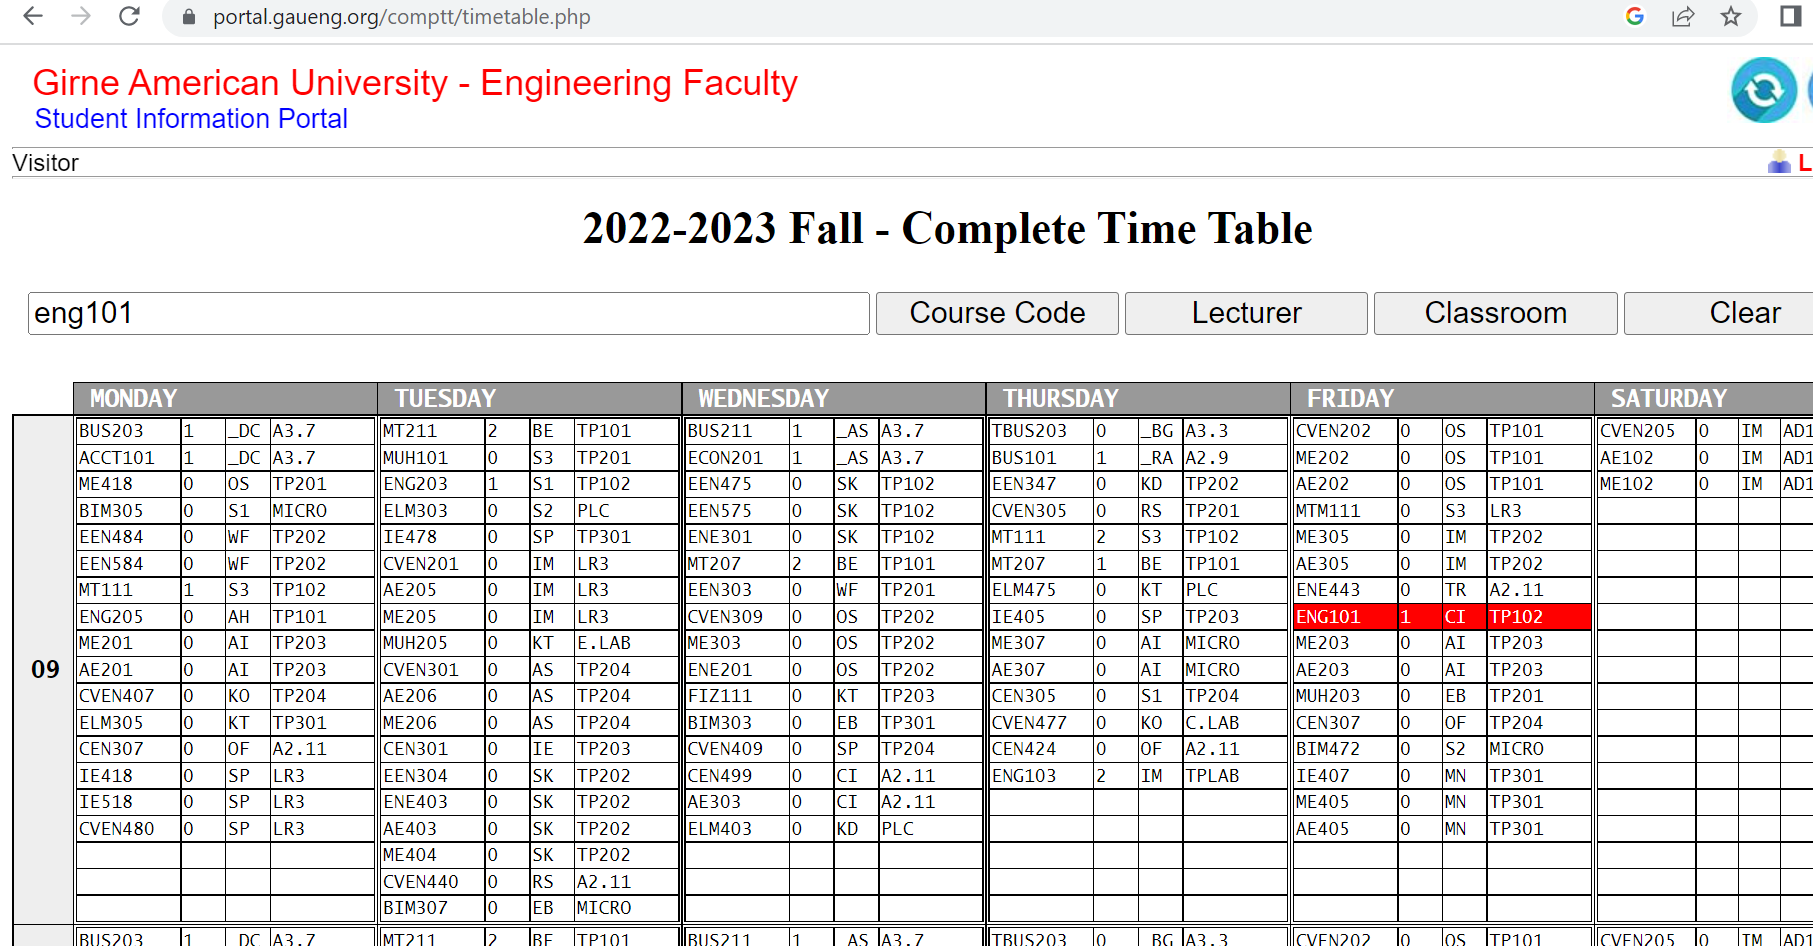
\includegraphics[width=\textwidth]{portal}
\end{figure}

\section{Testing}



\subsection{Letter grades}

\begin{table}[H]
	\centering
	\begin{tabular}{lll}
			\toprule
			Letter Grade & Score Interval & Coefficient\\
			\midrule
			A & 90-100 & 4.00\\
			A- & 85-89 & 3.70\\
			B+ & 80-84 & 3.30\\
			B & 75-79 & 3.00\\
			B- & 70-74 & 2.70\\
			C+ & 65-69 & 2.30\\
			C & 60-64 & 2.00\\
			C- & 55-59 & 1.70\\
			D+ & 50-54 & 1.30\\
			D & 45-49 & 1.00\\
			F & 0-44 & 0.00\\	
			NG (Nil grade) & - & 0.00\\	
			S (Satisfactory) & - & 0.00\\
			U (Unsatisfactory) & - & 0.00\\
			\bottomrule	
		\end{tabular}
\end{table}

\subsection{How do I check out exam grades?}

\begin{itemize}
	\item Visit student portal (\texttt{student.gau.edu.tr}).	
	\item Click \textit{My Courses} tab.
	\item Click \textit{Current Grades} to know your grades.
\end{itemize}

\subsection{How successful am I?}

\begin{itemize}
	\item After every semester, your Cumulative Grade Point Average (CGPA) is calculated based on your letter grades.
	\item The courses with higher credits will have more weight on your CGPA.
	\item Your CGPA is calculated out of 4.0. For example, if you get \textit{A} from all of your courses your CGPA will be 4.00 out of 4.00.
\end{itemize}

\subsection{How do I graduate?}

\begin{itemize}
	\item Each course has a credit. You will earn the credit by passing a course. Once you earn enough credits, you fulfill one the requirements to graduate. Visit specific department in \texttt{portal.gaueng.org/schedule} to see required credits to graduate. For example, for Computer Engineering you have to earn 132 credits.
	\item Keep your CGPA above 2.0. Students who plan to do Master and PhD degrees are encouraged to have at least 3.0 CGPA (2.5 for some universities) on graduation.
\end{itemize}

\subsection{Attending exams}

\begin{itemize}
	\item You need exam cards to attend midterm/final/make-up/resit exams.
	\item Get your exam card from faculty secretary.
\end{itemize}

\subsection{How do I follow announcements?}

\begin{itemize}
	\item Visit \texttt{portal.gaueng.org} frequently for announcements such as exam dates.
\end{itemize}







%\section{How do I find more information about lecturers?}
%
%\begin{itemize}
%\item Go to \url{portal.gaueng.org}
%\item Scroll down and click \textit{Staff} to get information about lecturers.
%\end{itemize}

\section{Online resources}

e-learning is useful to access online resources such as assignments and exams and also attending online classes and quizzes.

\subsection{Log in}

\begin{itemize}
	\item Visit \texttt{elearning.gau.edu.tr}.
	\item Click \textit{Log in} in upper right corner.
	\item Use student email address and password to log in.
\end{itemize}

\subsection{How to enroll in a course}

\begin{itemize}
	\item Visit \texttt{elearning.gau.edu.tr}.
	\item Scroll down and click \textit{Faculty of Engineering}.
\end{itemize}

\begin{figure}[H]
	\centering
	\begin{tikzpicture}
		\node at (0.0,0.0) {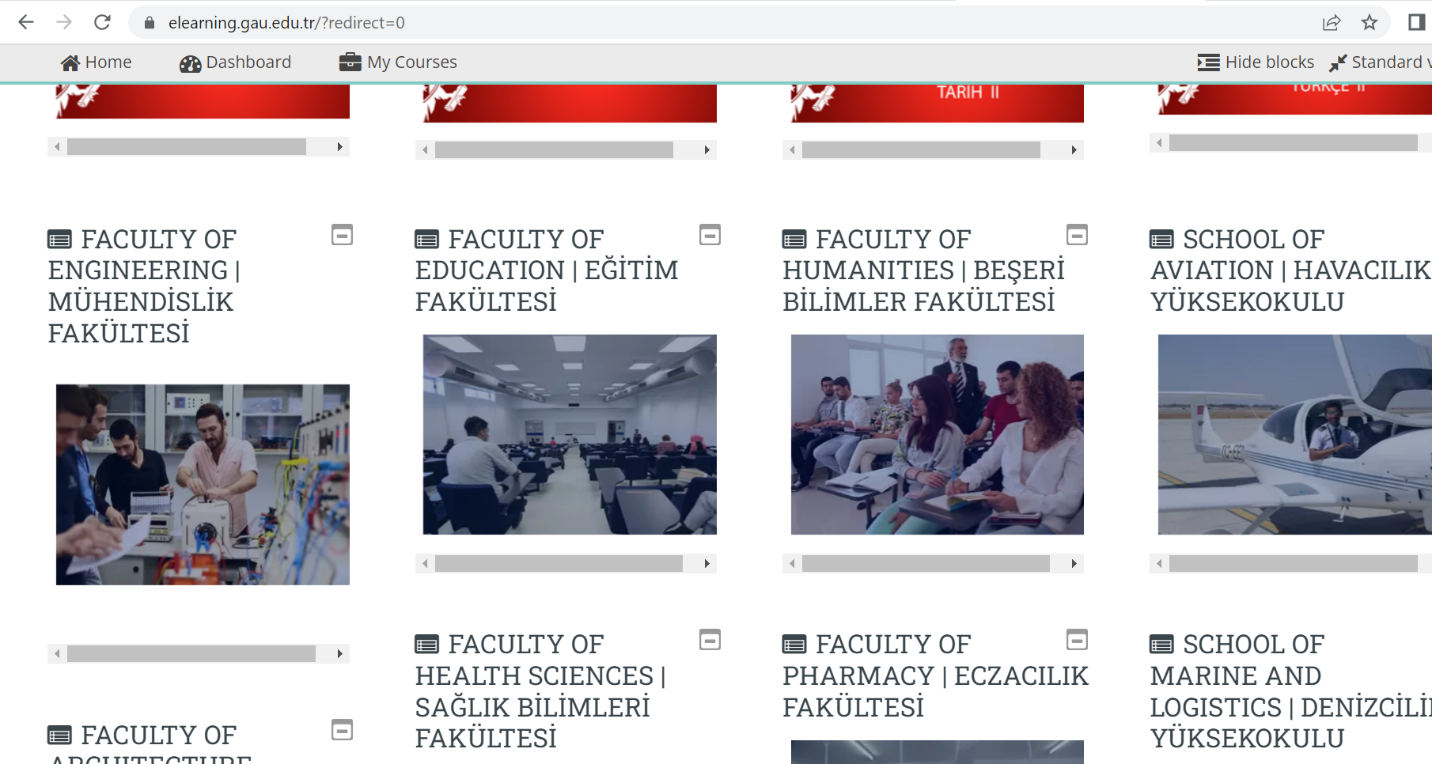
\includegraphics[width=\textwidth]{el1}};
		\draw[red] (-6.0,-2.0) rectangle (-3.0,1.7);
	\end{tikzpicture}	
\end{figure}

\begin{itemize}
	\item Search for name of the course you want to enroll in.
	\item In this example, name of the course is \textit{tfl101}.
\end{itemize}

\begin{figure}[H]
	\centering
	\begin{tikzpicture}
		\node at (0.0,0.0) {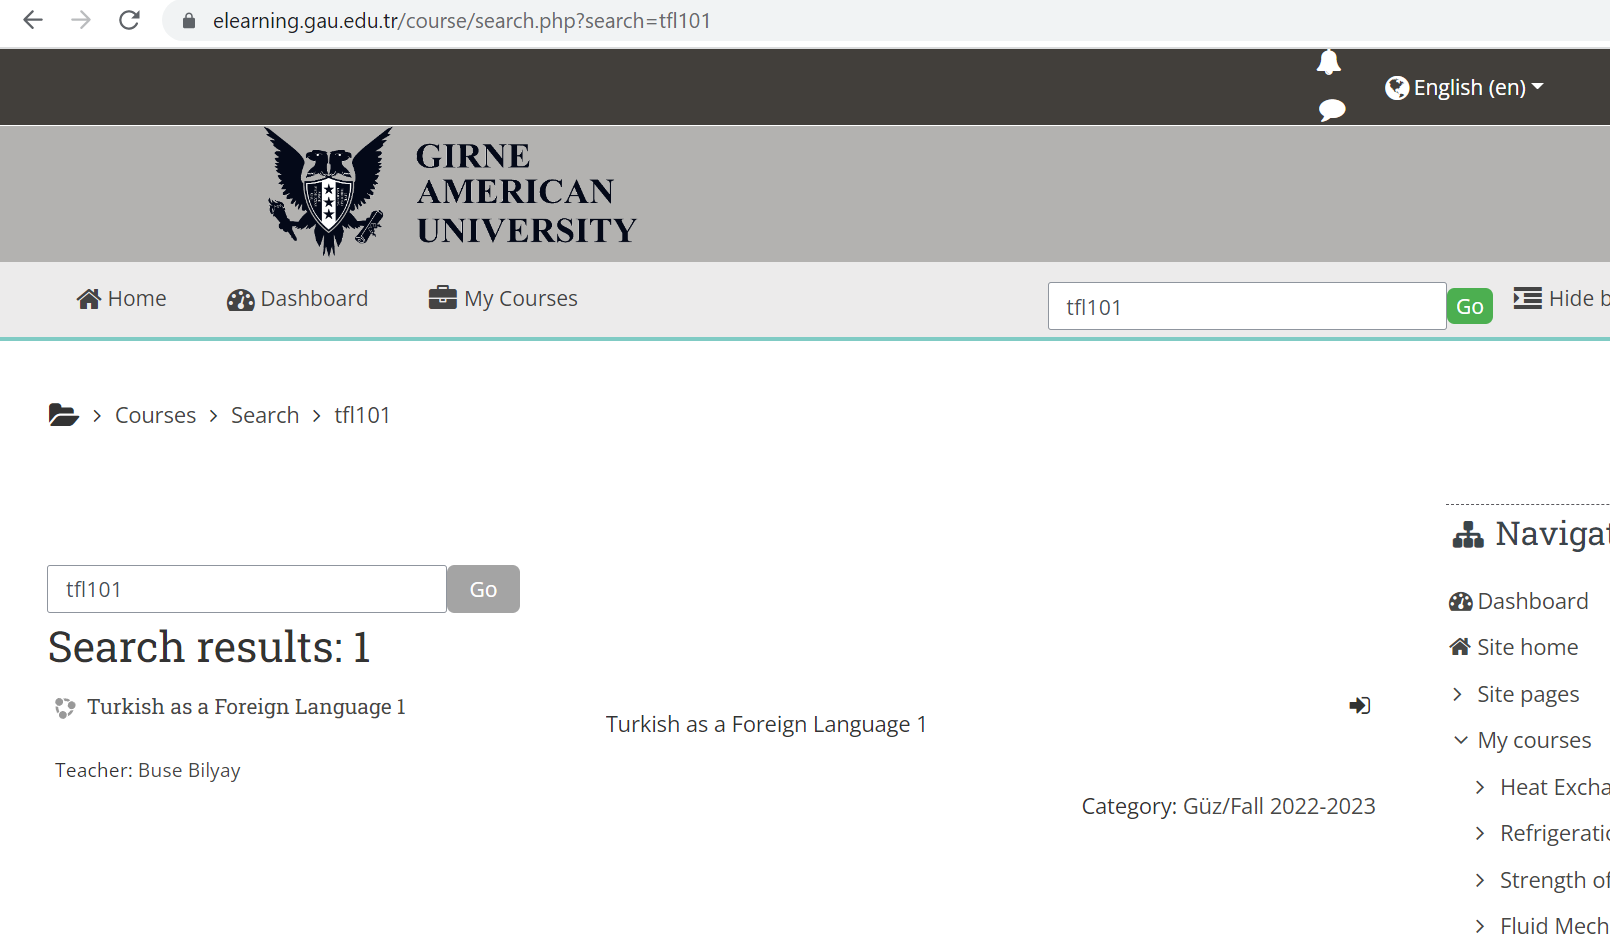
\includegraphics[width=\textwidth]{el2}};
		\draw[red] (-6.0,-1.1) rectangle (-2.0,-0.4);
	\end{tikzpicture}	
\end{figure}

\begin{itemize}
	\item Click \textit{Enroll me} button.
\end{itemize}

\begin{figure}[H]
	\centering
	\begin{tikzpicture}
		\node at (0.0,0.0) {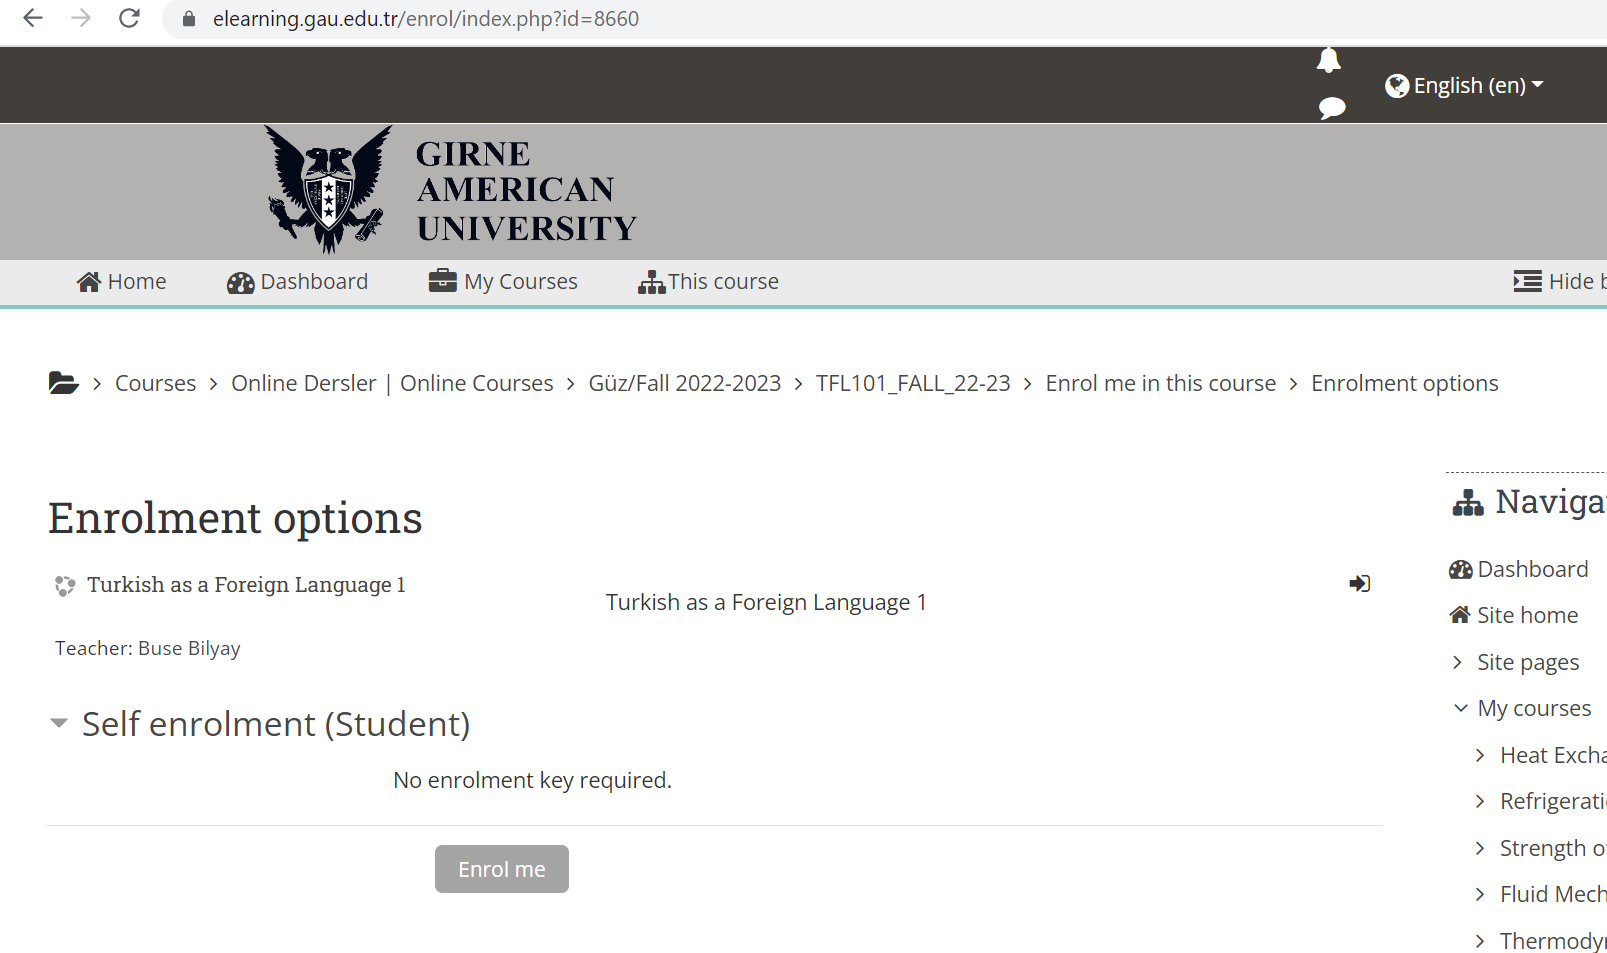
\includegraphics[width=\textwidth]{el3}};
		\draw[red] (-3.0,-3.3) rectangle (-1.5,-2.5);
	\end{tikzpicture}	
\end{figure}



\subsection{How do I attend TFL101 class?}

\begin{itemize}
	\item In order to join online classes, download and install \textit{Zoom}(\texttt{zoom.us}).
	\item Visit \texttt{elearning.gau.edu.tr}.
	\item Choose TFL101 in \textit{My Courses} drop down menu.
	\item Click the link provided by the lecturer.
\end{itemize}

\subsection{How TFL101 is graded?}

\begin{itemize}
	\item You either get \textit{S} (Satisfactory) or \textit{U} (Unsatisfactory).
\end{itemize}







\end{document}